\documentclass[12pt,letterpaper]{article}
\usepackage{fullpage}
\usepackage[top=2cm, bottom=4.5cm, left=2.5cm, right=2.5cm]{geometry}
\usepackage{amsmath,amsthm,amsfonts,amssymb,amscd}
\usepackage{lastpage}
\usepackage{tikz}
\usepackage{aeguill}
\usepackage{listings}
\usepackage{enumitem}
\usepackage{pgfplots}
\usepackage{fancyhdr}
\usepackage{mathrsfs}
\usepackage{mdframed}
\usepackage{xcolor}
\usepackage{graphicx}
\usepackage{listings}
\usepackage{hyperref}

\graphicspath{ {./images/} }
\setlength{\parindent}{0.0in}
\setlength{\parskip}{0.05in}
\definecolor{plantucolor0000}{RGB}{0,0,0}
\definecolor{plantucolor0001}{RGB}{255,255,255}
\definecolor{plantucolor0002}{RGB}{168,0,54}
\definecolor{plantucolor0003}{RGB}{254,254,206}
\definecolor{plantucolor0004}{RGB}{238,238,238}
% Edit these as appropriate
  
  \newcommand\course{CSCI 345}
  \newcommand\hwnumber{1}                  % <-- homework number
  \newcommand\NetIDa{Dan Aimone}           % <-- NetID of person #1
  \renewcommand{\labelenumii}{\theenumii}
  \renewcommand{\theenumii}{\theenumi.\arabic{enumii}.}
  % \newcommand\NetIDb{netid12038}           % <-- NetID of person #2 (Comment this line out for problem sets)

  \pagestyle{fancyplain}
  \headheight 35pt
  \lhead{\NetIDa}
  % \lhead{\NetIDa\\\NetIDb}                 % <-- Comment this line out for problem sets (make sure you are person #1)
  \chead{\textbf{\Large Assignment \hwnumber\;- Part 1}}
  \rhead{\course \\ \today}
  \lfoot{}
  \cfoot{}
  \rfoot{\small\thepage}
  \headsep 1.5em
  \mdfsetup{frametitlealignment=\center}

  \begin{document}
  \begin{mdframed}
  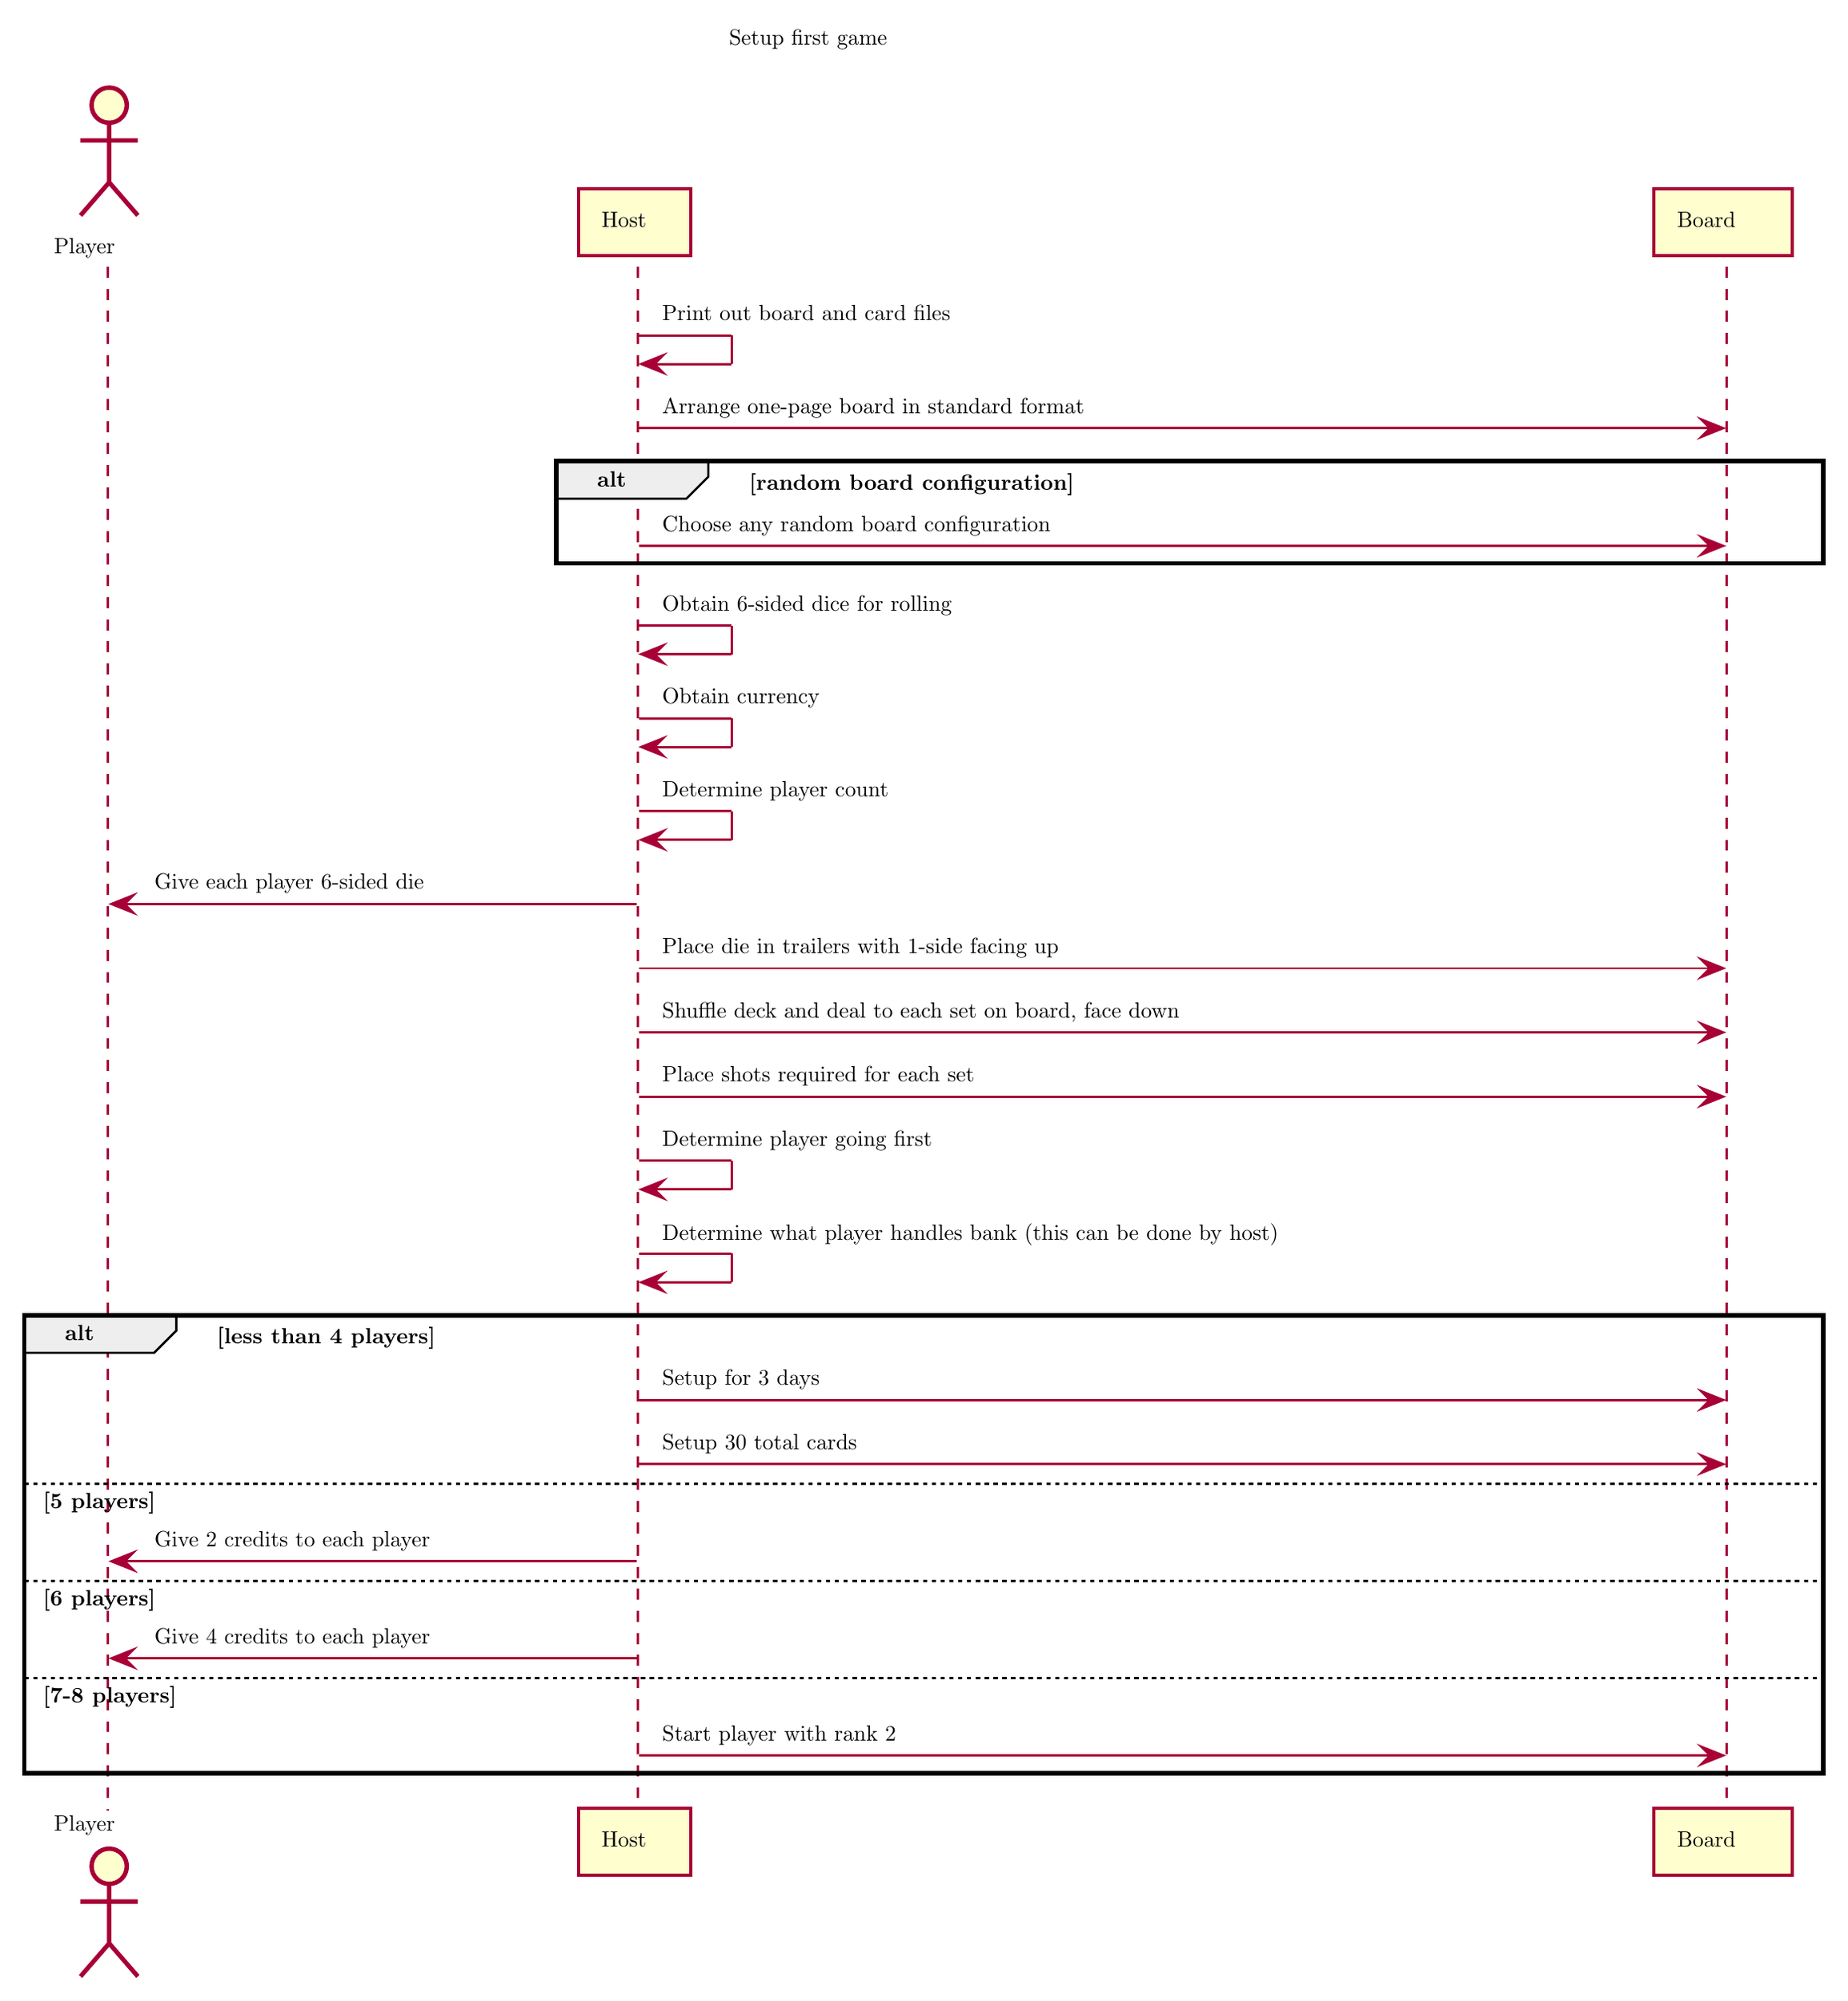
\begin{tikzpicture}[yscale=-1
  ,pstyle0/.style={color=black,fill=white,line width=2.0pt}
  ,pstyle1/.style={fill=white,color=white,line width=1.0pt}
  ,pstyle2/.style={color=plantucolor0002,line width=1.0pt,dash pattern=on 5.0pt off 5.0pt}
  ,pstyle3/.style={color=plantucolor0002,fill=plantucolor0003,line width=2.0pt}
  ,pstyle4/.style={color=plantucolor0002,line width=2.0pt}
  ,pstyle5/.style={color=plantucolor0002,fill=plantucolor0003,line width=1.5pt}
  ,pstyle6/.style={color=plantucolor0002,line width=1.0pt}
  ,pstyle7/.style={color=plantucolor0002,fill=plantucolor0002,line width=1.0pt}
  ,pstyle8/.style={color=black,fill=plantucolor0004,line width=1.0pt}
  ,pstyle9/.style={color=black,line width=2.0pt}
  ,pstyle10/.style={color=black,line width=1.0pt,dash pattern=on 2.0pt off 2.0pt}
  ]
  \node at (326.4892pt,12pt)[below right,color=black]{Setup first game};
  \draw[pstyle0] (251.6341pt,211.5156pt) rectangle (826.845pt,257.9209pt);
  \draw[pstyle0] (10pt,599.1162pt) rectangle (826.845pt,806.8213pt);
  \draw[pstyle1] (10pt,674.6543pt) rectangle (826.845pt,718.71pt);
  \draw[pstyle1] (10pt,718.71pt) rectangle (826.845pt,762.7656pt);
  \draw[pstyle1] (10pt,762.7656pt) rectangle (826.845pt,806.8213pt);
  \draw[pstyle2] (48pt,123.25pt) -- (48pt,823.8213pt);
  \draw[pstyle2] (288.6341pt,123.25pt) -- (288.6341pt,823.8213pt);
  \draw[pstyle2] (782.9688pt,123.25pt) -- (782.9688pt,823.8213pt);
  \node at (20pt,106.9531pt)[below right,color=black]{Player};
  \draw[pstyle3] (48.5778pt,49.9531pt) ellipse (8pt and 8pt);
  \draw[pstyle4] (48.5778pt,57.9531pt) -- (48.5778pt,84.9531pt)(35.5778pt,65.9531pt) -- (61.5778pt,65.9531pt)(48.5778pt,84.9531pt) -- (35.5778pt,99.9531pt)(48.5778pt,84.9531pt) -- (61.5778pt,99.9531pt);
  \node at (20pt,822.8213pt)[below right,color=black]{Player};
  \draw[pstyle3] (48.5778pt,849.1182pt) ellipse (8pt and 8pt);
  \draw[pstyle4] (48.5778pt,857.1182pt) -- (48.5778pt,884.1182pt)(35.5778pt,865.1182pt) -- (61.5778pt,865.1182pt)(48.5778pt,884.1182pt) -- (35.5778pt,899.1182pt)(48.5778pt,884.1182pt) -- (61.5778pt,899.1182pt);
  \draw[pstyle5] (261.6341pt,87.9531pt) rectangle (312.6887pt,118.25pt);
  \node at (268.6341pt,94.9531pt)[below right,color=black]{Host};
  \draw[pstyle5] (261.6341pt,822.8213pt) rectangle (312.6887pt,853.1182pt);
  \node at (268.6341pt,829.8213pt)[below right,color=black]{Host};
  \draw[pstyle5] (749.9688pt,87.9531pt) rectangle (812.845pt,118.25pt);
  \node at (756.9688pt,94.9531pt)[below right,color=black]{Board};
  \draw[pstyle5] (749.9688pt,822.8213pt) rectangle (812.845pt,853.1182pt);
  \node at (756.9688pt,829.8213pt)[below right,color=black]{Board};
  \draw[pstyle6] (289.1614pt,154.3828pt) -- (331.1614pt,154.3828pt);
  \draw[pstyle6] (331.1614pt,154.3828pt) -- (331.1614pt,167.3828pt);
  \draw[pstyle6] (290.1614pt,167.3828pt) -- (331.1614pt,167.3828pt);
  \draw[pstyle7] (300.1614pt,163.3828pt) -- (290.1614pt,167.3828pt) -- (300.1614pt,171.3828pt) -- (296.1614pt,167.3828pt) -- cycle;
  \node at (296.1614pt,137.25pt)[below right,color=black]{Print out board and card files};
  \draw[pstyle7] (771.4069pt,192.5156pt) -- (781.4069pt,196.5156pt) -- (771.4069pt,200.5156pt) -- (775.4069pt,196.5156pt) -- cycle;
  \draw[pstyle6] (289.1614pt,196.5156pt) -- (777.4069pt,196.5156pt);
  \node at (296.1614pt,179.3828pt)[below right,color=black]{Arrange one-page board in standard format};
  \draw[pstyle8] (251.6341pt,211.5156pt) -- (320.6341pt,211.5156pt) -- (320.6341pt,218.5156pt) -- (310.6341pt,228.5156pt) -- (251.6341pt,228.5156pt) -- (251.6341pt,211.5156pt);
  \draw[pstyle9] (251.6341pt,211.5156pt) rectangle (826.845pt,257.9209pt);
  \node at (266.6341pt,212.5156pt)[below right,color=black]{\textbf{alt}};
  \node at (335.6341pt,213.5156pt)[below right,color=black]{\textbf{[random board configuration]}};
  \draw[pstyle7] (771.4069pt,245.9209pt) -- (781.4069pt,249.9209pt) -- (771.4069pt,253.9209pt) -- (775.4069pt,249.9209pt) -- cycle;
  \draw[pstyle6] (289.1614pt,249.9209pt) -- (777.4069pt,249.9209pt);
  \node at (296.1614pt,232.7881pt)[below right,color=black]{Choose any random board configuration};
  \draw[pstyle6] (289.1614pt,286.0537pt) -- (331.1614pt,286.0537pt);
  \draw[pstyle6] (331.1614pt,286.0537pt) -- (331.1614pt,299.0537pt);
  \draw[pstyle6] (290.1614pt,299.0537pt) -- (331.1614pt,299.0537pt);
  \draw[pstyle7] (300.1614pt,295.0537pt) -- (290.1614pt,299.0537pt) -- (300.1614pt,303.0537pt) -- (296.1614pt,299.0537pt) -- cycle;
  \node at (296.1614pt,268.9209pt)[below right,color=black]{Obtain 6-sided dice for rolling};
  \draw[pstyle6] (289.1614pt,328.1865pt) -- (331.1614pt,328.1865pt);
  \draw[pstyle6] (331.1614pt,328.1865pt) -- (331.1614pt,341.1865pt);
  \draw[pstyle6] (290.1614pt,341.1865pt) -- (331.1614pt,341.1865pt);
  \draw[pstyle7] (300.1614pt,337.1865pt) -- (290.1614pt,341.1865pt) -- (300.1614pt,345.1865pt) -- (296.1614pt,341.1865pt) -- cycle;
  \node at (296.1614pt,311.0537pt)[below right,color=black]{Obtain currency};
  \draw[pstyle6] (289.1614pt,370.3193pt) -- (331.1614pt,370.3193pt);
  \draw[pstyle6] (331.1614pt,370.3193pt) -- (331.1614pt,383.3193pt);
  \draw[pstyle6] (290.1614pt,383.3193pt) -- (331.1614pt,383.3193pt);
  \draw[pstyle7] (300.1614pt,379.3193pt) -- (290.1614pt,383.3193pt) -- (300.1614pt,387.3193pt) -- (296.1614pt,383.3193pt) -- cycle;
  \node at (296.1614pt,353.1865pt)[below right,color=black]{Determine player count};
  \draw[pstyle7] (59.5778pt,408.4521pt) -- (49.5778pt,412.4521pt) -- (59.5778pt,416.4521pt) -- (55.5778pt,412.4521pt) -- cycle;
  \draw[pstyle6] (53.5778pt,412.4521pt) -- (288.1614pt,412.4521pt);
  \node at (65.5778pt,395.3193pt)[below right,color=black]{Give each player 6-sided die};
  \draw[pstyle7] (771.4069pt,437.585pt) -- (781.4069pt,441.585pt) -- (771.4069pt,445.585pt) -- (775.4069pt,441.585pt) -- cycle;
  \draw[pstyle6] (289.1614pt,441.585pt) -- (777.4069pt,441.585pt);
  \node at (296.1614pt,424.4521pt)[below right,color=black]{Place die in trailers with 1-side facing up};
  \draw[pstyle7] (771.4069pt,466.7178pt) -- (781.4069pt,470.7178pt) -- (771.4069pt,474.7178pt) -- (775.4069pt,470.7178pt) -- cycle;
  \draw[pstyle6] (289.1614pt,470.7178pt) -- (777.4069pt,470.7178pt);
  \node at (296.1614pt,453.585pt)[below right,color=black]{Shuffle deck and deal to each set on board, face down};
  \draw[pstyle7] (771.4069pt,495.8506pt) -- (781.4069pt,499.8506pt) -- (771.4069pt,503.8506pt) -- (775.4069pt,499.8506pt) -- cycle;
  \draw[pstyle6] (289.1614pt,499.8506pt) -- (777.4069pt,499.8506pt);
  \node at (296.1614pt,482.7178pt)[below right,color=black]{Place shots required for each set};
  \draw[pstyle6] (289.1614pt,528.9834pt) -- (331.1614pt,528.9834pt);
  \draw[pstyle6] (331.1614pt,528.9834pt) -- (331.1614pt,541.9834pt);
  \draw[pstyle6] (290.1614pt,541.9834pt) -- (331.1614pt,541.9834pt);
  \draw[pstyle7] (300.1614pt,537.9834pt) -- (290.1614pt,541.9834pt) -- (300.1614pt,545.9834pt) -- (296.1614pt,541.9834pt) -- cycle;
  \node at (296.1614pt,511.8506pt)[below right,color=black]{Determine player going first};
  \draw[pstyle6] (289.1614pt,571.1162pt) -- (331.1614pt,571.1162pt);
  \draw[pstyle6] (331.1614pt,571.1162pt) -- (331.1614pt,584.1162pt);
  \draw[pstyle6] (290.1614pt,584.1162pt) -- (331.1614pt,584.1162pt);
  \draw[pstyle7] (300.1614pt,580.1162pt) -- (290.1614pt,584.1162pt) -- (300.1614pt,588.1162pt) -- (296.1614pt,584.1162pt) -- cycle;
  \node at (296.1614pt,553.9834pt)[below right,color=black]{Determine what player handles bank (this can be done by host)};
  \draw[pstyle8] (10pt,599.1162pt) -- (79pt,599.1162pt) -- (79pt,606.1162pt) -- (69pt,616.1162pt) -- (10pt,616.1162pt) -- (10pt,599.1162pt);
  \draw[pstyle9] (10pt,599.1162pt) rectangle (826.845pt,806.8213pt);
  \node at (25pt,600.1162pt)[below right,color=black]{\textbf{alt}};
  \node at (94pt,601.1162pt)[below right,color=black]{\textbf{[less than 4 players]}};
  \draw[pstyle7] (771.4069pt,633.5215pt) -- (781.4069pt,637.5215pt) -- (771.4069pt,641.5215pt) -- (775.4069pt,637.5215pt) -- cycle;
  \draw[pstyle6] (289.1614pt,637.5215pt) -- (777.4069pt,637.5215pt);
  \node at (296.1614pt,620.3887pt)[below right,color=black]{Setup for 3 days};
  \draw[pstyle7] (771.4069pt,662.6543pt) -- (781.4069pt,666.6543pt) -- (771.4069pt,670.6543pt) -- (775.4069pt,666.6543pt) -- cycle;
  \draw[pstyle6] (289.1614pt,666.6543pt) -- (777.4069pt,666.6543pt);
  \node at (296.1614pt,649.5215pt)[below right,color=black]{Setup 30 total cards};
  \draw[pstyle10] (10pt,675.6543pt) -- (826.845pt,675.6543pt);
  \node at (15pt,675.6543pt)[below right,color=black]{\textbf{[5 players]}};
  \draw[pstyle7] (59.5778pt,706.71pt) -- (49.5778pt,710.71pt) -- (59.5778pt,714.71pt) -- (55.5778pt,710.71pt) -- cycle;
  \draw[pstyle6] (53.5778pt,710.71pt) -- (288.1614pt,710.71pt);
  \node at (65.5778pt,693.5771pt)[below right,color=black]{Give 2 credits to each player};
  \draw[pstyle10] (10pt,719.71pt) -- (826.845pt,719.71pt);
  \node at (15pt,719.71pt)[below right,color=black]{\textbf{[6 players]}};
  \draw[pstyle7] (59.5778pt,750.7656pt) -- (49.5778pt,754.7656pt) -- (59.5778pt,758.7656pt) -- (55.5778pt,754.7656pt) -- cycle;
  \draw[pstyle6] (53.5778pt,754.7656pt) -- (288.1614pt,754.7656pt);
  \node at (65.5778pt,737.6328pt)[below right,color=black]{Give 4 credits to each player};
  \draw[pstyle10] (10pt,763.7656pt) -- (826.845pt,763.7656pt);
  \node at (15pt,763.7656pt)[below right,color=black]{\textbf{[7-8 players]}};
  \draw[pstyle7] (771.4069pt,794.8213pt) -- (781.4069pt,798.8213pt) -- (771.4069pt,802.8213pt) -- (775.4069pt,798.8213pt) -- cycle;
  \draw[pstyle6] (289.1614pt,798.8213pt) -- (777.4069pt,798.8213pt);
  \node at (296.1614pt,781.6885pt)[below right,color=black]{Start player with rank 2};
  \end{tikzpicture}
  \end{mdframed}
  \end{document}

